\documentclass[aps,apl,twocolumn,groupedaddress]{revtex4-1}
%\documentclass[12pt]{article}   	% use "amsart" instead of "article" for AMSLaTeX format

\usepackage{color}
\usepackage{graphicx}				% Use pdf, png, jpg, or eps� with pdflatex; use eps in DVI mode
								% TeX will automatically convert eps --> pdf in pdflatex		
%\usepackage{caption}
\usepackage{soul}

\usepackage{natbib}
	
\newcommand{\CRout}[1]{\textcolor{blue}{\st{#1}}}
\newcommand{\CR}[1]{\textcolor{blue}{#1}}
\newcommand{\CRcomment}[1]{\textcolor{blue}{\textit{#1}}}

%\renewcommand{\CRout}[1]{}
%\renewcommand{\CR}[1]{{#1}}
%\renewcommand{\CRcomment}[1]{}

\begin{document}

\title{A Novel Route to Semi-Classic Quantum Mechanics \\ Or Maybe \\ Quantum Mechanics in the Semi-classical Regime}
\author{Chris Richardson, Peter Schlagheck, John Martin, Thierry Bastin}
\affiliation{University of Liege}
\date{\today}							% Activate to display a given date or no date

\begin{abstract}

We present a novel approach to explore semi-classical behavior based on a non-linear classical Schr\"{o}dinger-like equation which includes a classicality enforcing potential.  Scaling of this potential is shown to recover quantum behavior and is equivalent to scaling Planck's constant.

\end{abstract}

\maketitle

\section{Introduction}

The boundary between where quantum mechanics ends and classical mechanics begins is being pushed by experiments operating far from the microscopic scale in which quantum behavior is normally associated.  For example, Arndt \emph{et al}~\cite{bib:arndt} observed interference between mesoscopic fullerenes and Lee \emph{et al}'s~\cite{bib:leediamonds} experiment entangled the vibrational modes of two macroscopic diamonds.  It is important to be able to describe the manner in which quantum behavior transitions into classical behavior.  


Quantum mechanics is an extremely well tested theory and there is no doubt that all the behavior of classical mechanics is contained entirely within quantum theory.  A position reinforced by the Ehrenfest theorem which states that the expected mean values of measurement predicted from quantum mechanics obey classical Newtonian motion in the classical regime.  However, as quantum mechanics enters the transition area between the classical and quantum regimes, it becomes increasingly difficult to represent a quantum system using the full quantum formalism.  It is often unfeasible to model a complex or large quantum system without performing some sort of approximation such as WKB~\cite{bib:wkb} or Gross-Pitaevskii~\cite{bib:gpg,bib:gpp}.  We propose here a new approximation tool which can be used to describe the physical behavior of a system throughout the entire region between the quantum and classical regimes.

Despite classical non-relativistic mechanics being completely contained in non-relativistic quantum mechanics, they are discussed in quite different languages.  To develop a tool that smoothly transitions between the two regimes we must be able to describe them both using the same language.  Wavefunctions and wave equations are part of the language of quantum mechanics which is governed by the Schr\"{o}dinger wave equation,
\begin{eqnarray}
i \hbar \frac{\partial \psi(\mathbf{r},t)}{\partial t} = - \frac{\hbar^2}{2 m} \nabla^2 \psi(\mathbf{r},t) + V(\mathbf{r},t) \psi(\mathbf{r},t) \;, \label{eqn:schrod}
\end{eqnarray}
where $\psi$ is a wavefunction whose modulus squared gives a probability density of a particle, $m$ is the mass of the particle, $V$ is the potential experienced by the particle and $\hbar$ is the reduced Planck's constant.  Classical mechanics uses the language of trajectories and is governed by Newton's laws.  We can formulate classical mechanics so that all its behavior can be expressed by the Hamilton-Jacobi~\cite{bib:hamiltonjacobi} equation,
\begin{eqnarray}
\frac{\partial S_{c}(\mathbf{r},t)}{\partial t} &=& - \frac{1}{2 m} \left[\nabla S_{c}(\mathbf{r},t)\right]^2 - V(\mathbf{r},t) \;, \label{eqn:hamjac}
\end{eqnarray}
where $S_{c}$ is the classical action which defines a canonical transformation between initial and final phase-space coordinates.  For a given initial condition the behavior of a classical particle will be described by a trajectory derived from the action $S_{c}$.

The description of quantum mechanics using classical language has been well known since Madelung~\cite{bib:madelung} in 1926 and was rediscovered later by Bohm~\cite{bib:bohm} in 1952.  It begins by expressing the complex-valued wavefunction in its polar form,
\begin{eqnarray}
\psi(\mathbf{r},t) = A(\mathbf{r},t) e^{ i S(\mathbf{r},t) / \hbar } \;, \label{eqn:polarwf}
\end{eqnarray}
where $A$ is the real-valued amplitude and $S/\hbar$ is the real-valued phase.  Plugging this into the Schr\"{o}dinger equation, Eq. (\ref{eqn:schrod}), we obtain two equations.   The first is the continuity equation which describes the conservation of probability
\begin{eqnarray}
\frac{\partial A(\mathbf{r},t)}{\partial t} &=& - \frac{1}{m} \left[\nabla A(\mathbf{r},t)\right] \cdot [\nabla S(\mathbf{r},t)]  \label{eqn:continuity} \\
&-& \frac{1}{2 m} A(\mathbf{r},t) \nabla^2 S(\mathbf{r},t) \;, \nonumber
\end{eqnarray}
which is equivalent to $0 = \frac{\partial \rho}{\partial t} + \nabla \cdot \mathbf{j}$ where $\rho = \left| \psi \right|^2=  A^2$ and $\mathbf{j} = i \frac{\hbar}{2 m} (\psi^* \nabla \psi - \psi \nabla \psi^*) = -\frac{1}{m }A^2 \nabla S$ is the probability density current. The second is a Hamilton-Jacobi like equation
\begin{eqnarray}
\frac{\partial S(\mathbf{r},t)}{\partial t} &=& - \frac{1}{2 m} \left[\nabla S(\mathbf{r},t)\right]^2 - V(\mathbf{r},t) + U(\mathbf{r},t) \;. \label{eqn:hamjacbohm}
\end{eqnarray}
This equation differs in form from the Hamilton-Jacobi equation, Eq.~(\ref{eqn:hamjac}), by an extra potential,
 \begin{eqnarray}
U(\mathbf{r},t) &=& - \frac{\hbar^2}{2 m} \frac{ \nabla^2 A(\mathbf{r},t)}{A(\mathbf{r},t)} = - \frac{\hbar^2}{2 m} \frac{\nabla^2 \left| \psi(\mathbf{r},t) \right|}{\left| \psi(\mathbf{r},t) \right|}  \label{eqn:qmp}
\end{eqnarray}
which Bohm called the \emph{quantum-mechanical potential}.  Adding this potential to the classical Hamilton-Jacobi, Eq. (\ref{eqn:hamjac}), allows us to derive an action which in turn gives a trajectory.  However unlike a classical trajectory this one can have quantum behavior and non-Newtonian motion.

The description of classical mechanics using quantum language is less well known.  Following Oriols and Mompart~\cite{bib:obm} we describe an ensemble of initial positions by the distribution $A_c^2(\mathbf{r},0)$.  The trajectories resulting from these initial positions will evolve according to the Hamilton-Jacobi equation and give $A_c^2(\mathbf{r},t)$, which can be seen as describing the probability distribution of a particle at time $t > 0$.  A classical wavefuction similar to Eq.~(\ref{eqn:polarwf}), $\psi_{c}(\mathbf{r},t) = A_{c}(\mathbf{r},t) \exp\left[i S_{c}(\mathbf{r},t) / \hbar\right]$, can be constructed where $\hbar$ is used to provide a dimensionless argument and $S_{c}$ is again the classical action from the Hamilton-Jacobi equation, Eq.~(\ref{eqn:hamjac}).  Using this form of the wavefunction Oriols and Mompart~\cite{bib:obm} derive a wave equation, similar in form to the Schr\"{o}dinger equation, that describes the evolution of a classical particle.  We call it the classical Schr\"{o}dinger-like equation and it is given by
\begin{eqnarray}
i \hbar \frac{\partial \psi_{c}(\mathbf{r},t)}{\partial t} &=& - \frac{\hbar^2}{2 m} \nabla^2 \psi_{c}(\mathbf{r},t) + V(\mathbf{r},t) \psi_{c}(\mathbf{r},t) \label{eqn:class_schrod} \\ 
&+& \frac{\hbar^2}{2 m} \frac{\nabla^2 \left| \psi_{c}(\mathbf{r},t) \right|}{\left| \psi_{c}(\mathbf{r},t) \right|} \psi_{c}(\mathbf{r},t) \;, \nonumber 
\end{eqnarray}
where the probability density is given from the modulus squared, $\rho_c = \left|\psi_{c}\right|^2$, of the wavefunction in analogy to quantum mechanics, is .  Eq.~(\ref{eqn:class_schrod}) while having completely classical behavior is similar in form to the Schr\"{o}dinger equation except for an extra non-linear term which has the effect of canceling out all quantum or wave-like effects.  Schleich \emph{et al.}~\cite{bib:revisited} refer to this term as the \emph{classicality-enforcing potential} and it is of course Bohm's quantum-mechanical potential, Eq.~(\ref{eqn:qmp}), with the opposite sign, $-U(\mathbf{r},t)$.  They transfer from the non-linear classical Schr\"{o}dinger-like equation, Eq.~(\ref{eqn:class_schrod}),  to the linear Schr\"{o}dinger equation, Eq.~(\ref{eqn:schrod}), by first making the anzatz $\psi_{c} = \psi$.   They then define a \emph{quantum action} which includes the classicality-enforcing potential.  This leads to the cancelation of the classicality-enforcing potential in Eq.~(\ref{eqn:class_schrod}) and recovery of the Schr\"{o}dinger equation and quantum mechanics.  Schleich \emph{et al.}~\cite{bib:revisited} claim that to recover quantum mechanics Eq.~(\ref{eqn:class_schrod}) must become linear but we will show here that it is not necessary to completely cancel out the classicality-enforcing potential to recover quantum behavior.  We find that by scaling and not necessarily eliminating the classicality-enforcing potential we can reproduce quantum behavior and recover the linear Schr\"{o}dinger equation with a rescaled Planck's constant.

We choose here to use the language of quantum mechanics and describe both regimes using wavefunctions and wave equations.  This allows us to explore how to transition between the two regimes using consistent language.  We insert a \emph{degree of quantumness} $\epsilon$ where $0 \leq \epsilon \leq 1$, into Eq.~(\ref{eqn:class_schrod}) which modulates the classicality-enforcing potential.  
\begin{eqnarray}
i \hbar \frac{\partial \psi(\mathbf{r},t)}{\partial t} &=& - \frac{\hbar^2}{2 m} \nabla^2 \psi(\mathbf{r},t) + V(\mathbf{r},t) \psi(\mathbf{r},t) \label{eqn:class_schrod_ep} \\ 
&+& (1 - \epsilon) \frac{\hbar^2}{2 m} \frac{\nabla^2 \left| \psi(\mathbf{r},t) \right|}{\left| \psi(\mathbf{r},t) \right|} \psi(\mathbf{r},t) \nonumber
\end{eqnarray}
We call this the \emph{transition equation} and we will show that it exhibits quantum behavior.  The transition equation is equal to the Schr\"{o}dinger equation for $\epsilon = 1$ and equal to the non-linear classical Schr\"{o}dinger-like equation for $\epsilon = 0$.  For all other values $0 < \epsilon < 1$ this non-linear equation behaves in the same manner as the linear Schr\"{o}dinger equation.  To demonstrate this we take two approaches.  First in Sec.~\ref{sec:scaling} we show analytically that the transition equation is equivalent to the Schr\"{o}dinger equation with a rescaled $\hbar$.  We then in Sec.~\ref{sec:inter} explore numerically what the effect of scaling the classicality-enforcing potential has on the interference of two Gaussian wave packets.

\section{Equivalence to Scaling Planck's Constant\label{sec:scaling}}

The non-linear transition equation can be shown to be equivalent to the linear Schr\"{o}dinger equation with Planck's constant scaled by the degree of quantumness according to
\begin{eqnarray}
\tilde{\hbar} = \hbar \sqrt{\epsilon} \;. \label{eqn:hbar_scaled}
\end{eqnarray}

We insert the polar form of the wavefunction, Eq.~(\ref{eqn:polarwf}), into the transition equation, Eq.~(\ref{eqn:class_schrod_ep}), and find the individual elements.
\begin{eqnarray}
\nabla^2 \psi(\mathbf{r},t) &=& \Big\{ \nabla^2 A(\mathbf{r},t) + 2 \frac{i}{\hbar}  [\nabla A(\mathbf{r},t)] \cdot [\nabla S(\mathbf{r},t)]  \label{eqn:cont_laplacian}  \\
&+& \frac{i}{\hbar} A(\mathbf{r},t) \nabla^2 S(\mathbf{r},t) - \frac{1}{\hbar^2}  A(\mathbf{r},t) [\nabla S(\mathbf{r},t)]^2 \Big\} \nonumber \\
&\times& e^{ i S(\mathbf{r},t) / \hbar } \nonumber \;,  \\
i \hbar \frac{\partial \psi(\mathbf{r},t)}{\partial t} &=& \left[i \hbar \frac{\partial A(\mathbf{r},t)}{\partial t} - A \frac{\partial S(\mathbf{r},t)}{\partial t}\right] e^{ i S(\mathbf{r},t) / \hbar } \;, \label{eqn:cont_polar}
\end{eqnarray}
\begin{eqnarray}
\frac{\psi(\mathbf{r},t)}{\left| \psi(\mathbf{r},t) \right|} \nabla^2 \left| \psi(\mathbf{r},t) \right| &=& [\nabla^2 A(\mathbf{r},t)] e^{ i S(\mathbf{r},t) / \hbar } \;, \label{eqn:cont_cp}
\end{eqnarray}
where Eq.~(\ref{eqn:cont_laplacian}) is the Laplacian, Eq.~(\ref{eqn:cont_polar}) is time derivative of the polar wavefunction and Eq.~(\ref{eqn:cont_cp}) is the contribution from the classicality-enforcing potential.

Gathering the real and imaginary terms we obtain the continuity equation, Eq.~(\ref{eqn:continuity}), and an equation very similar to the Hamilton-Jacobi equation, Eq.~(\ref{eqn:hamjac}).  It differs from it by the addition of Bohm's quantum-mechanical potential scaled by the degree of quantumness,
\begin{eqnarray}
 \frac{\partial S(\mathbf{r},t)}{\partial t} &=& - \frac{1}{2 m} [\nabla S(\mathbf{r},t)]^2 \nonumber \\
 &-& \left[V(\mathbf{r},t) - \epsilon \frac{\hbar^2}{2 m} \frac{ \nabla^2 A(\mathbf{r},t)}{A(\mathbf{r},t)}\right] \;.
\end{eqnarray}

This equation can be made to have the appearance of the Schr\"{o}dinger equation by making the substitution $\tilde{\hbar} = \hbar \sqrt{\epsilon}$.   Performing this substitution yields
\begin{eqnarray}
\frac{\partial S(\mathbf{r},t)}{\partial t} &=& - \frac{1}{2 m} [\nabla S(\mathbf{r},t)]^2 \label{eqn:hamilton-jacobi_rescaled} \\
&-& \left[V(\mathbf{r},t) - \frac{\tilde{\hbar}^2}{2 m} \frac{ \nabla^2 A(\mathbf{r},t)}{A(\mathbf{r},t)}\right] \;, \nonumber
\end{eqnarray}
by which means the degree of quantumness is cancelled out.  Eqs.~(\ref{eqn:continuity}) and (\ref{eqn:hamilton-jacobi_rescaled}) are now completely equivalent to the Schr\"{o}dinger equation with a rescaled $\hbar$ and we can write a scaled Schr\"{o}dinger-like equation and the associated wavefunction
\begin{eqnarray}
\tilde{\psi}(\mathbf{r},t) &\equiv& A(\mathbf{r},t) e^{i S(\mathbf{r},t) / \tilde{\hbar}} \label{eqn:tildewf} \\
&=& \psi(\mathbf{r},t) e^{i S(\mathbf{r},t) (1 / (\hbar \sqrt{\epsilon}) - 1 / \hbar)} \;, \\
i \tilde{\hbar} \frac{\partial \tilde{\psi}(\mathbf{r},t)}{\partial t}  &=& -  \frac{\tilde{\hbar}^2}{2 m} \nabla^2 \tilde{\psi}(\mathbf{r},t) + V(\mathbf{r},t) \tilde{\psi}(\mathbf{r},t) \;.
\end{eqnarray}
and note that $| \tilde{\psi}(\mathbf{r},t)|^2 = | \psi(\mathbf{r},t)|^2$.  We also note that as $\tilde{\hbar} \rightarrow 0$ the phase of Eq.~\ref{eqn:tildewf} will begin to vary rapidly compared to its amplitude.  This is a necessary assumption of the WKB approximation~\cite{bib:wkb} which leads to accurate results in the semi-classical regime away from the classical turning points.
 
\section{The Interference of Two Wave Packets\label{sec:inter}}

Using quantum mechanics we would expect two wave packets to spread with time and be represented by the standard Young interference pattern~\cite{bib:Young}.  For classical particles with no wave nature we expect the packets to maintain their shape and not interfere for all time.  We can explore the transition between these two extremes by solving the non-linear transition equation numerically.  For comparison, we first solve the system using the Schr\"{o}dinger equation.

\subsection{Quantum Wave Packet Behavior}

\begin{figure}[ht]
\begin{minipage}{0.25\textwidth}
  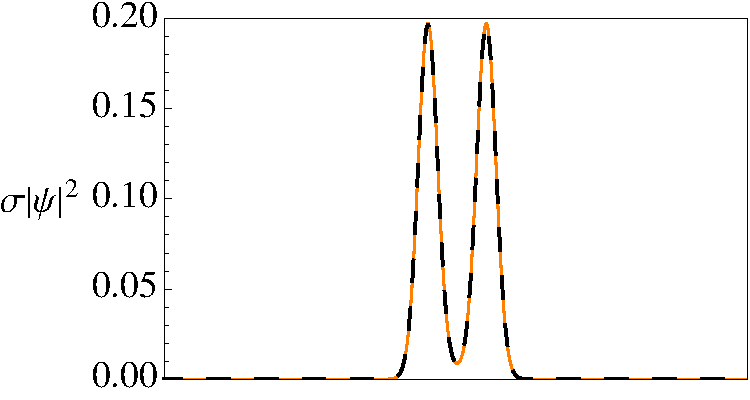
\includegraphics[width=1\textwidth]{Graphics/ProbsV_ep-10.pdf}
\end{minipage}
\begin{minipage}{0.2\textwidth}
  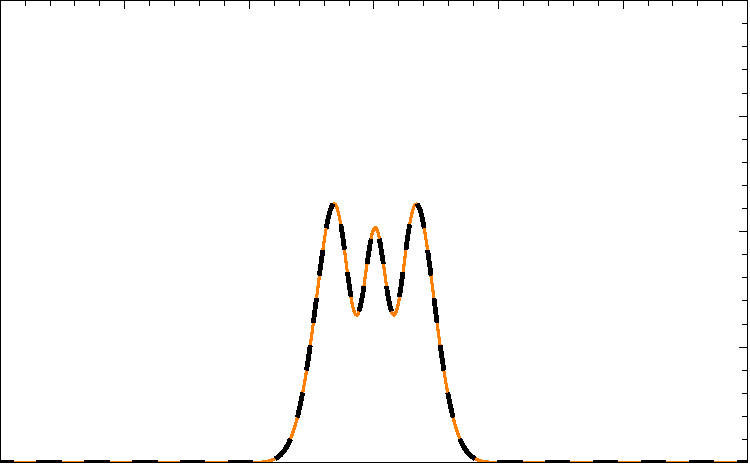
\includegraphics[width=1\textwidth]{Graphics/ProbsV_ep-98.pdf}
\end{minipage}
\begin{minipage}{0.25\textwidth}
  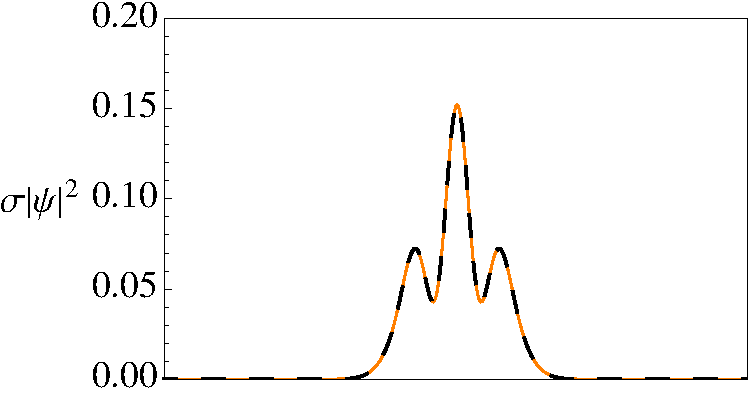
\includegraphics[width=1\textwidth]{Graphics/ProbsV_ep-95.pdf}
\end{minipage}
\begin{minipage}{0.2\textwidth}
  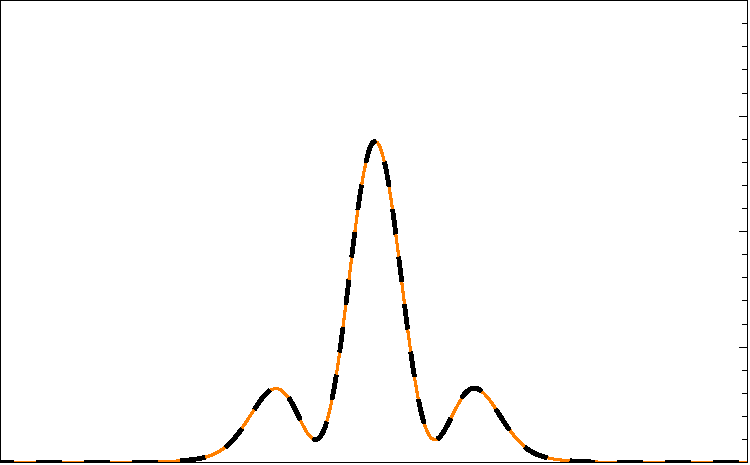
\includegraphics[width=1\textwidth]{Graphics/ProbsV_ep-8.pdf}
\end{minipage}
\begin{minipage}{0.25\textwidth}
  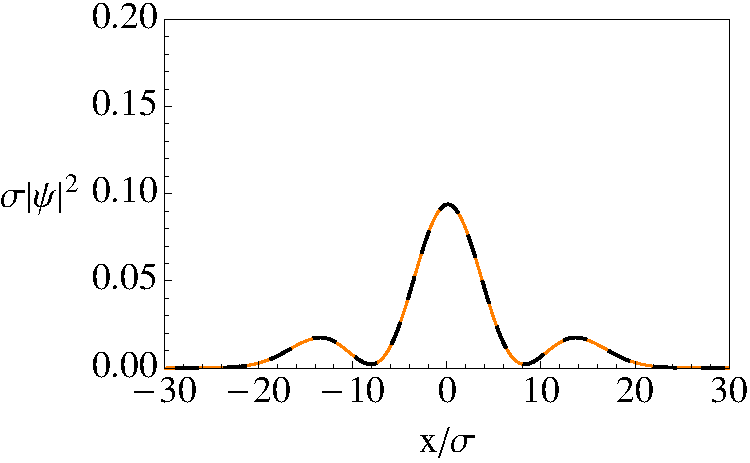
\includegraphics[width=1\textwidth]{Graphics/ProbsV_ep-4.pdf}
\end{minipage}
\begin{minipage}{0.2\textwidth}
  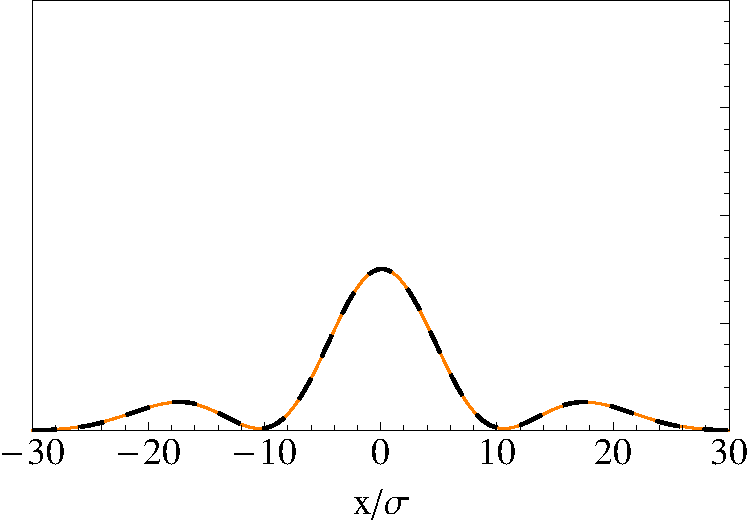
\includegraphics[width=1\textwidth]{Graphics/ProbsV_ep-0.pdf}
\end{minipage}
\caption{Solid line is the analytic probability density using the Schr\"{o}dinger equation with a scaled $\hbar = \tilde{\hbar} \sqrt{\epsilon}$ and the dashed line is the simulated probability density using the transition equation.  All plots are evaluated at the same time $t = 20 m \sigma^2 / \hbar$ and the distance between the center of the two gaussians is $d = 6 \sigma$. Plot (a) is the fully classical case with $\epsilon = 0$. (b) $\epsilon = 0.02$. (c) $\epsilon = 0.05$. (d) $\epsilon = 0.2$. (e) $\epsilon = 0.6$. (f) is for the case $\epsilon = 1$ when $\tilde{\hbar} = \hbar$.}
\label{fig:diffract_movie}
\end{figure}

%\begin{figure*}[ht]
%\begin{minipage}[t]{0.32\textwidth}
%%\centering
%  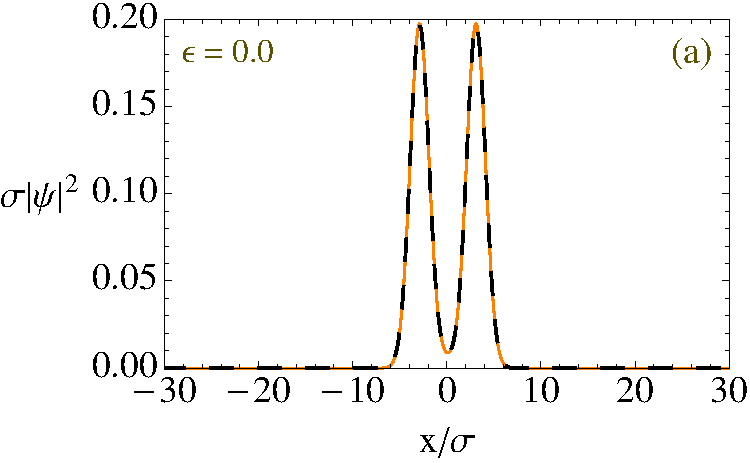
\includegraphics[width=1\textwidth]{Graphics/Probs_ep-10.pdf}
%  %\caption*{(a)}
%\end{minipage}
%\begin{minipage}[t]{0.32\textwidth}
%%\centering
%  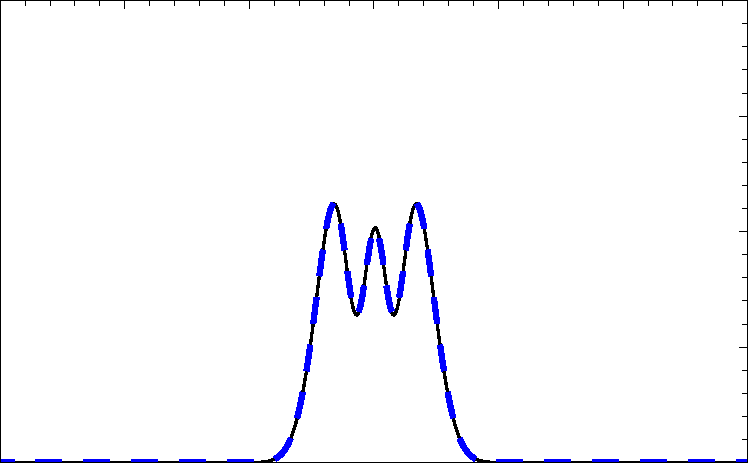
\includegraphics[width=1\textwidth]{Graphics/Probs_ep-98.pdf}
%  %\caption*{(b)}
%\end{minipage}
%\begin{minipage}[t]{0.32\textwidth}
%%\centering
%  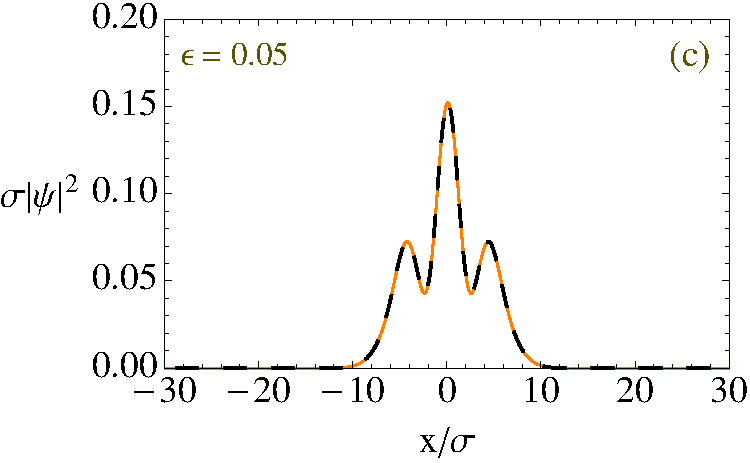
\includegraphics[width=1\textwidth]{Graphics/Probs_ep-95.pdf}
%  %\caption*{(c)}
%\end{minipage}
%\begin{minipage}[t]{0.32\textwidth}
%%\centering
%  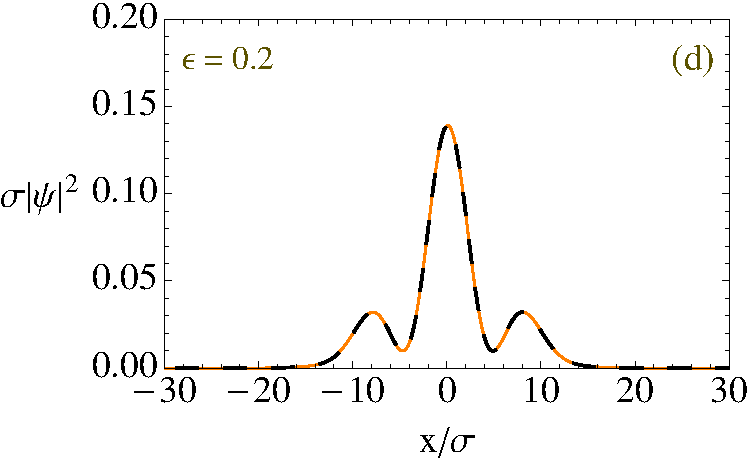
\includegraphics[width=1\textwidth]{Graphics/Probs_ep-8.pdf}
%  %\caption*{(d)}
%\end{minipage}
%\begin{minipage}[t]{0.32\textwidth}
%%\centering
%  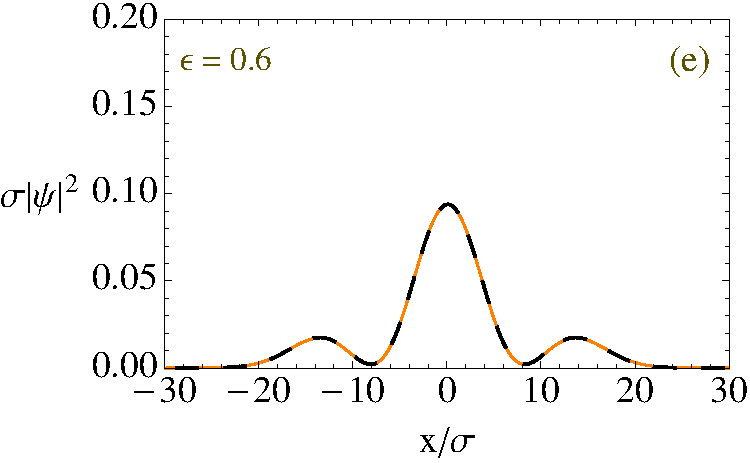
\includegraphics[width=1\textwidth]{Graphics/Probs_ep-4.pdf}
%  %\caption*{(e)}
%\end{minipage}
%\begin{minipage}[t]{0.32\textwidth}
%%\centering
%  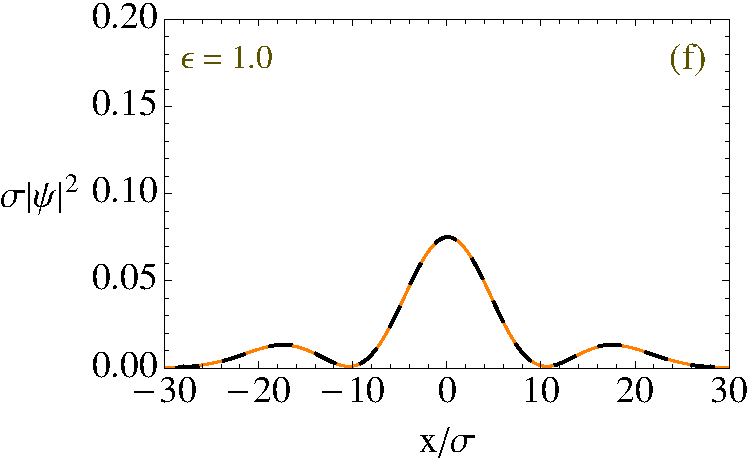
\includegraphics[width=1\textwidth]{Graphics/Probs_ep-0.pdf}
%  %\caption*{(f)}
%\end{minipage}
%\caption{Solid line is the analytic probability density using the Schr\"{o}dinger equation with a scaled $\hbar = \tilde{\hbar} \sqrt{\epsilon}$ and the dashed line is the simulated probability density using the transition equation.  All plots are evaluated at the same time $t = 20 m \sigma^2 / \hbar$ and the distance between the center of the two gaussians is $d = 6 \sigma$. Plot (a) is the fully classical case with $\epsilon = 0$. (b) $\epsilon = 0.02$. (c) $\epsilon = 0.05$. (d) $\epsilon = 0.2$. (e) $\epsilon = 0.6$. (f) is for the case $\epsilon = 1$ when $\tilde{\hbar} = \hbar$.}
%\label{fig:diffract_movie}
%\end{figure*}

We start the quantum analysis with two gaussians in one dimension with $V = 0$ and initial condition
\begin{eqnarray}
\psi(x,0) &=& \sqrt{N_0} \left\{ \exp[-\frac{(x-d)^2}{4 \sigma^2}]+\exp[-\frac{(x+d)^2}{4 \sigma ^2}]\right\} \label{eqn:double_init}
\end{eqnarray}
where $d$ is the distance from the origin to the centers of the Gaussians and $\sigma$ is the root mean square (rms) width. The normalization is
\begin{eqnarray}
 N_0 = \left[2 \sqrt{2 \pi } \sigma  \left(e^{-\frac{d^2}{2 \sigma ^2}}+1\right)\right]^{-1} \;.
 \end{eqnarray}

Solving the one dimensional time-dependent Schr\"{o}dinger equation,
\begin{eqnarray}
i \hbar \frac{\partial \psi}{\partial t} &=& -\frac{\hbar^2}{2 m} \frac{\partial^2 \psi}{\partial x^2} \;,
\end{eqnarray}
for this initial condition, the time-dependent wave function is found to be
\begin{eqnarray}
\psi(x,t) &=& \sqrt{\frac{N_0}{a_t}} \left(e^{-\frac{(x-d)^2}{4 a^2_t}}+e^{-\frac{(x+d)^2}{4 a^2_t}}\right) \;.
\end{eqnarray}
where $a^2_t =  \sigma^2 + \frac{1}{2} i \hbar t / m$.  When the modulus is squared the interference term becomes obvious,

\begin{eqnarray}
\left| \psi(x,t) \right|^2 &=& \frac{N_0}{\sigma_t} \Bigg[\left(e^{-\frac{(x-d)^2}{4 \sigma^2_t}}+e^{-\frac{(x+d)^2}{4 \sigma^2_t}}\right)^2 \label{eqn:wf_double_t}  \\
&-& 4 e^{-\frac{ \left(x^2 + d^2\right)}{2 \sigma^2_t}} \sin^2 \left(\frac{\hbar}{4 m \sigma^2 \sigma^2_t} t x d \right)\Bigg]\nonumber
\end{eqnarray}
where $\sigma^2_t = \hbar^2 t^2 / \left(4 m^2 \sigma^2\right) +\sigma^2$ is the time dependent rms width.  This gives the expected Young interference pattern.

\subsection{Simulation of Semi-Quantum Semi-Classical Wave Packets}

To explore the transitional behavior of the interference of two Gaussian wave packets from the quantum to the classical regime we use the transition equation, Eq.~(\ref{eqn:class_schrod_ep}), in one dimension and with $V = 0$
\begin{eqnarray}
i \hbar \frac{\partial \psi(x,t)}{\partial t} &=& -\frac{\hbar^2}{2 m} \frac{\partial^2 \psi(x,t)}{\partial x^2} \nonumber \\
&+& \frac{\hbar^2}{2 m} \frac{1 - \epsilon}{\left| \psi(x,t) \right|} \frac{\partial^2 \left| \psi(x,t) \right|}{\partial x^2} \psi(x,t) \;.  \label{eqn:schrod_class_nov}
\end{eqnarray}
We solve this equation numerically using the explicit finite difference method.  The asymptotic behavior is as expected.  For the case in which $\epsilon = 1$ and $\tilde{\hbar} = \hbar$ the interference pattern that forms, Fig.~\ref{fig:diffract_movie}(f), is identical to the analytic case, Eq.~(\ref{eqn:wf_double_t}).  For the case in which $\epsilon = 0$ and $\tilde{\hbar} = 0$ the interference pattern that forms, Fig.~\ref{fig:diffract_movie}(a), is just that of the initial distribution, Eq.~(\ref{eqn:double_init}).  As can be seen in all the frames of Fig.~\ref{fig:diffract_movie} for all values of $\epsilon$ the numerically solved non-linear transition equation is equivalent to the linear Schr\"{o}dinger equation with a scaled $\hbar$

For all values of $0 < \epsilon \leq 1$ an interference pattern develops.  Given enough time the pattern will develop into the usual far-field Young interference pattern with a visibility of one.  As can be seen in Fig.~\ref{fig:diffract_movie} the time for a diffraction pattern to develop increases to infinity as degree of quantumness diminishes.  The only value in which no interference is observed is that for $\epsilon = 0$.  When using the transition equation classical mechanics is a special singular case.

\section{Conclusion}
We have demonstrated both analytically and numerically that it is not necessary to get rid of the classicality-enforcing potential appearing in Oriols and Mompart's~\cite{bib:obm} classical Schr\"{o}dinger-like equation to recover behavior similar to that of quantum mechanics.  We have found that by using a degree of quantumness to scale but not necessarily eliminate the classicality-enforcing potential quantum behavior is observed and the linear Schr\"{o}dinger equation is recovered but with a rescaled Planck's constant.  This is used to define the transition equation which gives us a new tool to explore the transition area between the classical and quantum regimes.

It is interesting that the special behavior observed in the linear theory of quantum mechanics can be reproduced with a non-linear wave equation such as the transition equation.  It has been well proven~\cite{bib:qmlinear} that quantum mechanics is linear and so too is the transition equation when the degree of quantumness equal to one.  However when the degree of quantumness is anywhere between zero and one, where non-linearity is introduced, quantum behavior is still observed.  The non-linear transition equation mimics the linear Schr\"{o}dinger equation.  This may be why pure classical mechanics is only observed for the singular case when the degree of quantumness vanishes completely.

\CRcomment{Conclusion is too short imho, but I've said what I want to say.  We could elaborate of the singularity of classical mechanics or on how the nonlinear transition equation mimics the Schr\"{o}dinger equation but I am not sure why else to say about it.}


%It is also interesting that pure classical mechanics is only observed for the singular case when the degree of quantumness vanishes completely.  It is more natural to have quantum effects than not.  This is evident when observing the microscopic world as it is very difficult to avoid quantum effects.  It is less obvious for macroscopic experiments, where quantum behavior should be absent.  When these macroscopic experiments are considered in the light of the transition equation it should be noted that quantum behavior is almost never absent and it only needs be teased out.  For experiments that operate in the transition area it is therefore not necessary to make a one-to-one correspondence with quantum mechanics to demonstrate quantum behavior.  The transition equation allows a relaxation of the requirements that an experiment would have abide by the Schr\"{o}dinger equation to be able to say with certainty that quantum behavior was observed.

\begin{acknowledgments}
We would like to thank the Action de Recherche Concert�e (ARC) for funding and the rest of the Quandrops team.
\end{acknowledgments}

\bibliography{Biblio}

%\begin{thebibliography}{4}
%
%\bibitem{bib:arndt}
%M. Arndt, O. Nairz, J. Vos-Andreae, C. Keller, G. van der Zouw, and A. Zeilinger, \emph{Wave-particle duality of C60 molecules}, Nature 401, 680, (1999).
%
%\bibitem{bib:leediamonds}
%K. C. Lee1, M. R. Sprague, B. J. Sussman, J. Nunn, N. K. Langford, X.-M. Jin, T. Champion, P. Michelberger, K. F. Reim, D. England, D. Jaksch, I. A. Walmsley \emph{Entangling Macroscopic Diamonds at Room Temperature}, Science 334,1253, (2011).
%
%\bibitem{bib:wkb}
%Sakurai, J. J., \emph{Modern Quantum Mechanics. Addison-Wesley}, (1993).
%
%\bibitem{bib:gpg}
%Gross, E.P. \emph{Structure of a quantized vortex in boson systems}. Il Nuovo Cimento 20 (3): 454�457, (1961).
%
%\bibitem{bib:gpp}
% Pitaevsk, L. P.  \emph{Vortex Lines in an Imperfect Bose Gas}. Soviet Physics JETP 13 (2): 451�454, (1961).
%
%%\bibitem{bib:newton}
%%Newton, Isaac, \emph{Philosophiae Naturalis Principia Mathematica}, London, (1687).
%
%\bibitem{bib:hamiltonjacobi}
%Landau, L. D. and Lifshitz, E. M., \emph{Mechanics}, Pergamon Press, Oxford, (1969).
%
%\bibitem{bib:madelung}
%E. Madelung, \emph{Quantentheorie in hydrodynamischer}. Z Phys 40:322�326, (1926).
%
%\bibitem{bib:bohm}
%D. Bohm, \emph{A Suggested Interpretation of the Quantum Theory in Terms of ``Hidden'' Variables}. I, Phys. Rev. 85, 166, (1952).
%
%\bibitem{bib:obm}
%X.Oriols and J.Mompart \emph{Overview of Bohmian Mechanics}pages: 15-147; Chapter 1 of the book \emph{Applied Bohmian Mechanics: From Nanoscale Systems to Cosmology} Editorial Pan Stanford Publishing Pte. Ltd (2012).
%
%\bibitem{bib:revisited}
%Wolfgang P. Schleich, Daniel M. Greenberger, Donald H. Kobe, and Marlan O. Scully
%\emph{Schr\"{o}dinger equation revisited}
%PNAS 110 (14) 5374-5379, (2013).
%
%\bibitem{bib:Young}
%Thomas Young, \emph{Experimental Demonstration of the General Law of the Interference of Light}, Philosophical Transactions of the Royal Society of London, vol 94, (1804).
%
%%\bibitem{bib:macent}
%%S. Ghosh, T. F. Rosenbaum, G. Aeppli and S. N. Coppersmith, \emph{Entangled quantum state of magnetic dipoles}, Nature 425 48, (2003).
%
%\bibitem{bib:qmlinear}
%Urbasi Sinha, Christophe Couteau, Thomas Jennewein, Raymond Laflamme, Gregor Weihs, \emph{Ruling Out Multi-Order Interference in Quantum Mechanics}, Science 329, 418, (2010).
%
%%\bibitem{bib:couder_orbits}
%%E. Fort, A. Eddi, A. Boudaoud, J. Moukhtar, and Y. Couder, \emph{Path-memory induced quantization of classical orbits}, PNAS 107, 17515 (2010).
%%
%%\bibitem{bib:theonlymystery}
%%Feynman, Richard P. \emph{Six Easy Pieces} Reading, MA: Addison-Wesley, 1995.
%
%\end{thebibliography}


\end{document}  